% Created 2017-07-19 on. 14:17
% Intended LaTeX compiler: pdflatex
\documentclass[11pt]{article}
\usepackage[utf8]{inputenc}
\usepackage[T1]{fontenc}
\usepackage{graphicx}
\usepackage{grffile}
\usepackage{longtable}
\usepackage{wrapfig}
\usepackage{rotating}
\usepackage[normalem]{ulem}
\usepackage{amsmath}
\usepackage{textcomp}
\usepackage{amssymb}
\usepackage{capt-of}
\usepackage{hyperref}
\date{19 juli 2017}
\title{Åpne Rmd fil i riktig enkoding format}
\hypersetup{
 pdfauthor={Yusman Kamaleri},
 pdftitle={Åpne Rmd fil i riktig enkoding format},
 pdfkeywords={},
 pdfsubject={},
 pdfcreator={Emacs 25.1.1 (Org mode 9.0.9)}, 
 pdflang={Norsk}}
\begin{document}

\maketitle
\section*{UTF-8}
\label{sec:orgaa8b581}
Valg fil som skal åpnes i \texttt{RStudio}. Når filen er åpen, så skal den re-åpnes med riktig
enkoding format for at norske bokstaver skal leses riktig.  \\

For å gjøre det, valg \texttt{File} og så \texttt{Reopen with Encoding}. Deretter valg \texttt{UTF-8}. Bilder nedenfor viser disse

\begin{center}
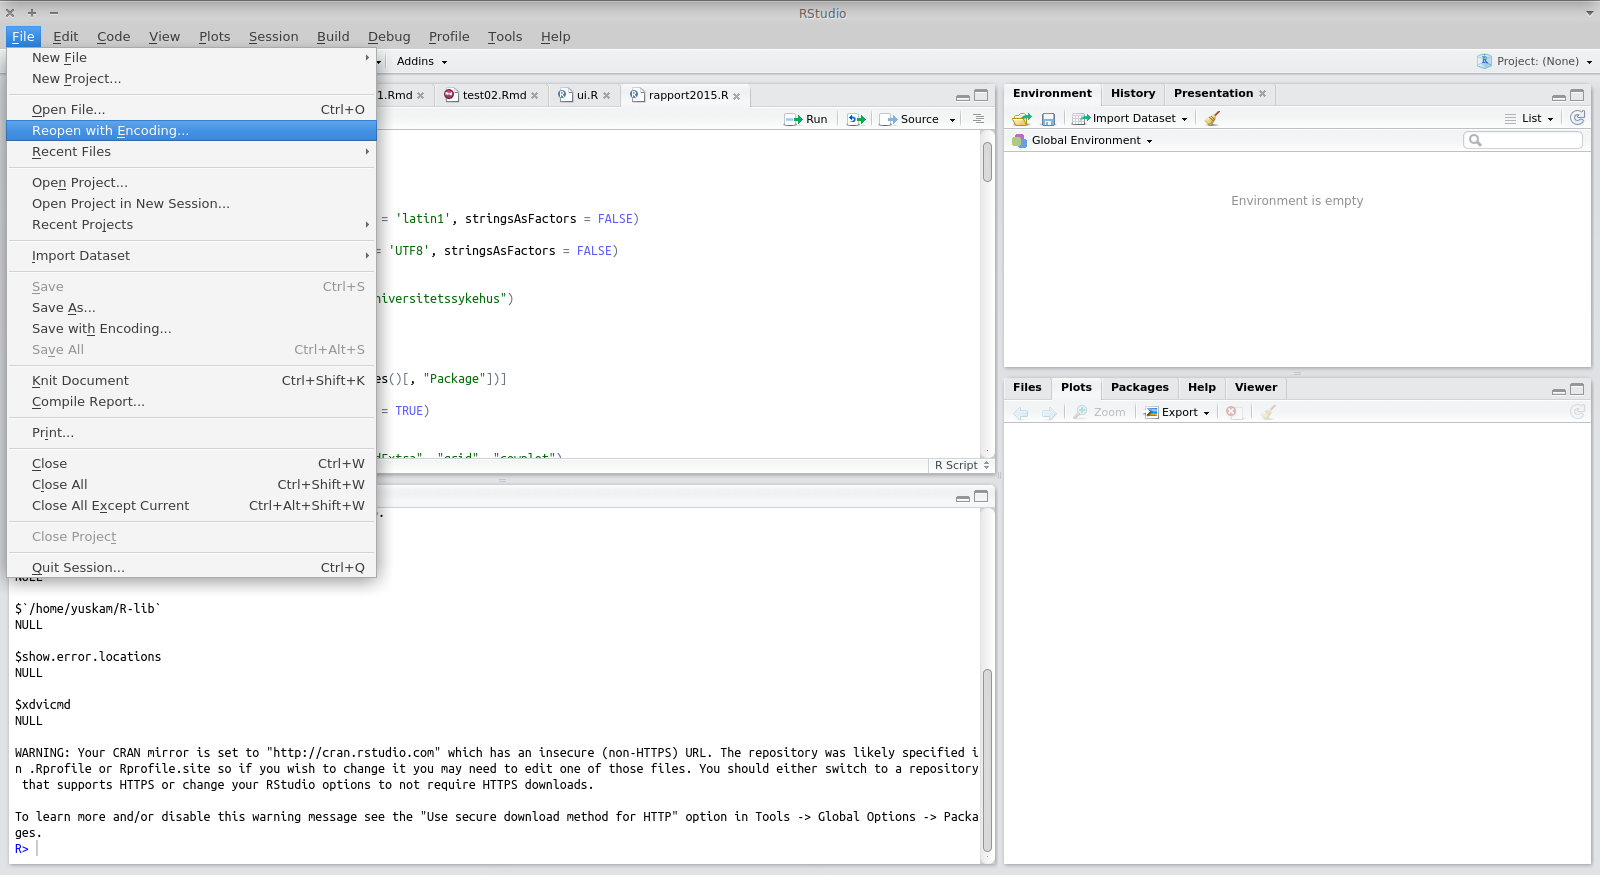
\includegraphics[width=15cm]{./utf8v2.png}
\end{center}
\end{document}